\documentclass[11pt]{article}
\usepackage[utf8]{inputenc}
\usepackage{geometry}
\geometry{a4paper, margin=1in}
\usepackage{graphicx}
\usepackage{hyperref}
\usepackage{booktabs}
\usepackage{subcaption}

\title{Analysis of Consumer Financial Fraud and Prevention Strategies \\
\large CIS 3319: Wireless Networks and Security / CIS 4378: Computer and Network Security \\
\large Lab 1: Consumer Financial Fraud Investigation}
\author{Group Members: \\ Aaron Jefferson \\ }
\date{01-Feb-2024}

\begin{document}

\maketitle

\begin{abstract}
\noindent This report provides an analysis of consumer financial fraud, including key findings and conclusions drawn from studying various cases and prevention strategies. The cases were selected from the Darknet Diaries podcast. 
\end{abstract}

\tableofcontents

\section{Introduction}
The purpose of this report is to provide an focused high level analysis of consumer financial fraud, highlighting the importance of understanding how the fraud took place, and the methodology used in the investigation.

\section{Exploration of Consumer Financial Fraud}
\subsection{Examples and Analysis}

\begin{figure}[ht]
    \centering
    \begin{subfigure}{.3\textwidth}
      \centering
      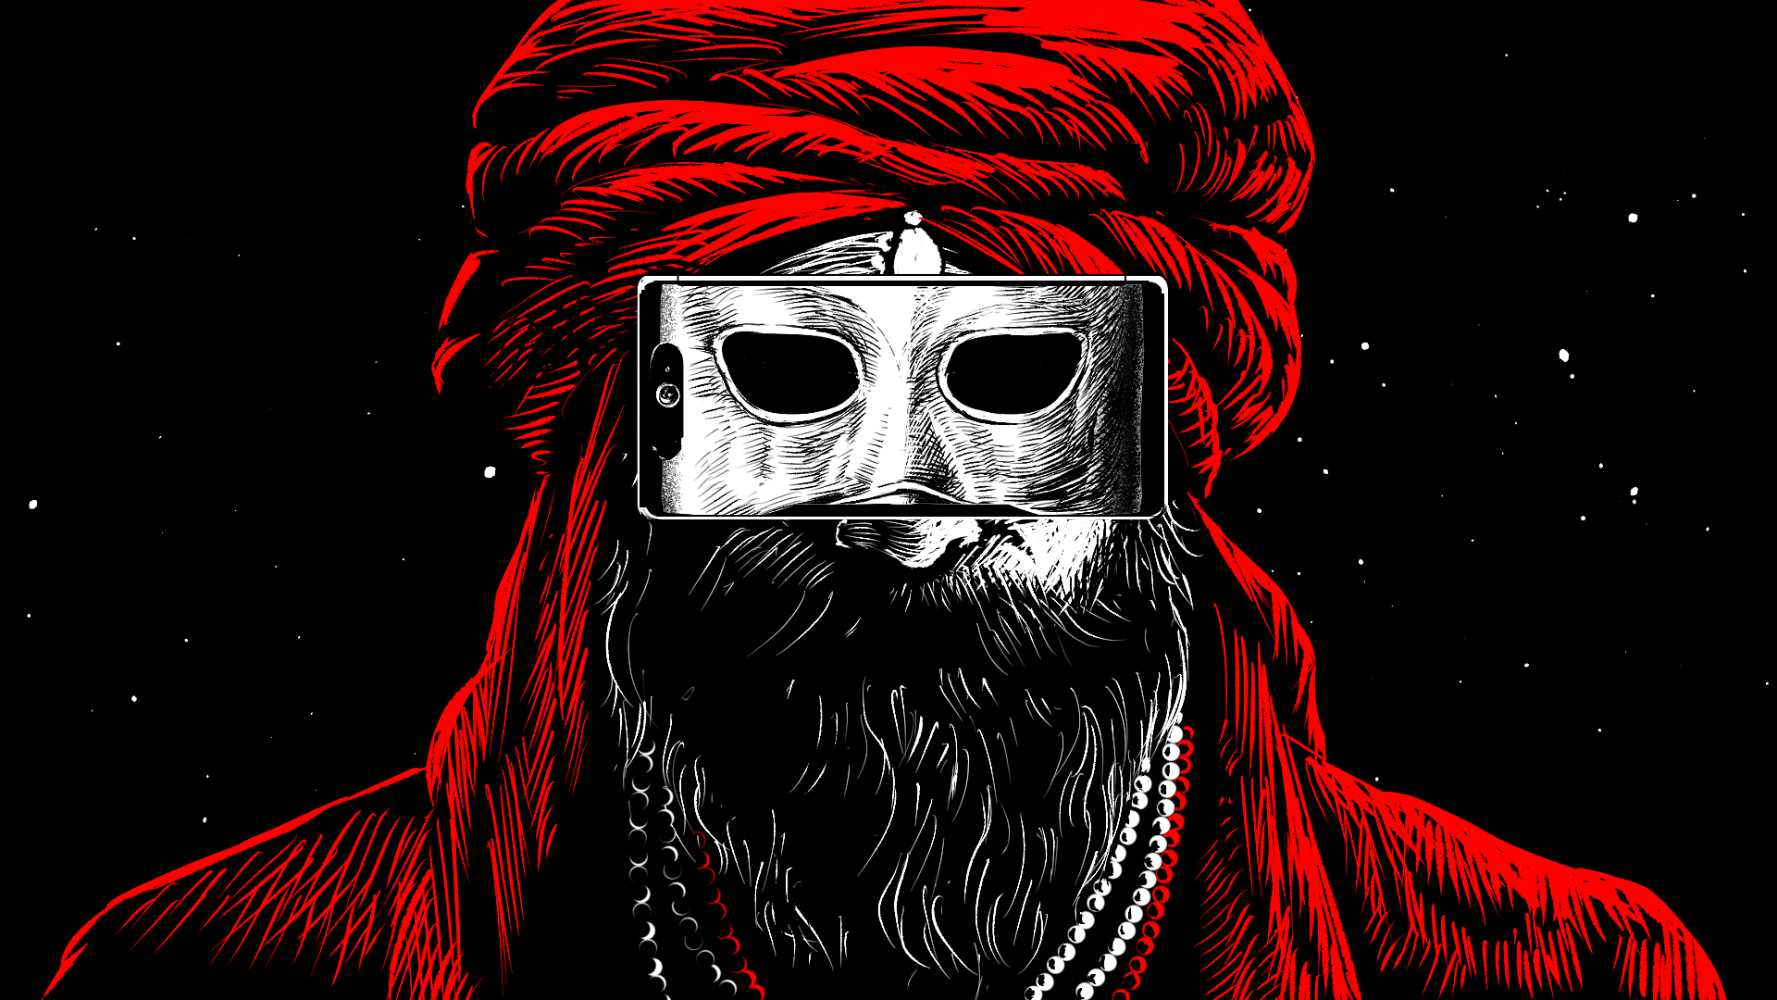
\includegraphics[width=\linewidth]{maskedphone.jpg}
      \caption{WhatsApp Fraud: Mimics}
      \label{fig:sub1}
    \end{subfigure}%
    \begin{subfigure}{.3\textwidth}
      \centering
      
\includegraphics[width=\linewidth]{wires.jpg}
      \caption{Stock Market Manipulation: Newswires}
      \label{fig:sub2}
    \end{subfigure}
    \begin{subfigure}{.3\textwidth}
      \centering
      
\includegraphics[width=\linewidth]{whale.jpg}
      \caption{Financial Deception: Impersonation and fake invoices}
      \label{fig:sub3}
    \end{subfigure}
    \caption{Visual Representations of Financial Fraud Cases}
    \label{fig:test}
    \end{figure}

\begin{tabular}{@{}llll@{}}
\toprule
\textbf{Source} & \textbf{Brief Description} & \textbf{Vulnerabilities} & \textbf{Attack Vectors} \\ \midrule
\textit{WhatsApp Fraud} & A case of social engineering where victims are deceived into financial loss through WhatsApp communications. & Trust exploitation, lack of digital literacy & Impersonation, phishing messages \\
\textit{WhatsApp Fraud} & A case of social engineering where victims are deceived into financial loss through WhatsApp communications. & Trust exploitation, lack of digital literacy & Impersonation, phishing messages \\
\textit{WhatsApp Fraud} & A case of social engineering where victims are deceived into financial loss through WhatsApp communications. & Trust exploitation, lack of digital literacy & Impersonation, phishing messages \\
% Add more rows and figures as needed
\bottomrule
\end{tabular}

Discuss each example in detail, focusing on how the fraud was perpetrated.

\subsection{Common Vulnerabilities and Attack Vectors}
Summarize the common vulnerabilities and attack vectors identified in the examples.

\section{Prevention Advice Analysis}
\subsection{Examples of Advice}
\begin{tabular}{@{}ll@{}}
\toprule
\textbf{Source} & \textbf{Advice} \\ \midrule
www.example.com & 1. Advice 1 \\ 
                & 2. Advice 2 \\
% Add more rows as needed
\bottomrule
\end{tabular}

Discuss each piece of advice, ensuring clarity for a general audience.

\subsection{Summary of Common Advice}
Summarize the common pieces of advice identified.

\section{Effectiveness of Prevention Strategies}
\subsection{Analysis of Advice Against Vulnerabilities}
Assess how each piece of advice addresses the vulnerabilities and attack vectors.

\subsection{Limitations and Unaddressed Threats}
Identify any advice that does not target vulnerabilities or attack vectors, and highlight any attacks not defended by the advice.

\subsection{Tailoring Advice for Specific Populations}
Discuss how advice might need modification for older adults, non-native English speakers, visually impaired users, etc.

\section{Conclusion}
Summarize the key findings, the effectiveness of current advice, and any recommendations for improvement.

\section{References}
List all sources used in your report.

\end{document}
